\chapter{Empirisk analyse}
I dette kapitel anvender vi data fra FRED, som er hentet fra Federal Reserve Bank of St. Louis \url{https://research.stlouisfed.org/econ/mccracken/fred-databases/}.
Der anvendes nogle transformationer for at gøre tidsrækkerne stationære, som er noteret mere detaljeret i appendiks ... 
Disse transformationer er forslået af Michael McCracken fra Federal Reserve Bank of St. Louis.  
Der observeres at 5 af disse variabler har mere end 43 NA's inkluderet og derfor bliver de fjernet fra datasættet. 
Derudover ser vi at de resterende NA's opstår kun i de første eller/og sidste observationer, vi fjerner derfor 17 observationer i hver variable for at undgå NA's. 
Så vores datasæt inkluderer altså 123 tidsrækker, som indeholder $691$ månedlige observationer og går fra 1. januar 1960 til 1. juli 2017. 
Hernæst har vi standardiseret vores data, således at variablerne er centreret omkring 0 og har en varians 1, således vi undgår skæringen i vores regression. 

Datasættet repræsenterer en stor brede af makroøkonomiske variabler, som Michael McCracken har inddelt i 8 kategorier. 
\begin{itemize}
\item \textbf{Output og indkomst:} Indeholder 16 tidsrækker
\item \textbf{Arbejdsmarked:}  Indeholder 31 tidsrækker
\item \textbf{Boliger:} Indeholder 10 tidsrækker
\item \textbf{Forbrug, ordrer og varebeholdninger:} Indeholder 7 tidsrækker
\item \textbf{Penge og kredit:} Indeholder 14 tidsrækker
\item\textbf{ Rente og valutakurs:} Indeholder 21 tidsrækker
\item \textbf{Priser:} Indeholder 20 tidsrækker
\item \textbf{Aktiemarked:} Indeholder 4 tidsrækker
\end{itemize}

Når vi konstruerer vores model anvender vi 122 forklarende variabler og 1 respons variable og for at validerer vores model deler vi vores fulde datasæt i et træningssæt, som består af 552 observationer fra 1. januar 1960 til 1. december 2005 og et testsæt, som består af 139 observationer fra 1. januar 2006 til 1. Juli 2017. 
En betydningsfuld makroøkonomisk variable er arbejdsløshed, som blandt andet vil være vores responsvariable.  Arbejdsløshed er inkluderet i gruppen arbejdsmarked. 
\section{Benchmark}
Faktormodellen


\section{Shrinkage metoder}
I denne sektion vil vi finde den optimale $\lambda$ for de forskellige shrinking metoder. 
Vi har tidligere introduceret to algoritmer til at løse vores optimerings problemer, som vi vil anvende i denne sektion.
Vi deler derfor vores analyse op i to dele, hvor vi anvender hhv. coordinate descent og LARS algoritmen.

Metoderne er alle anvendt med forskellige værdier af $\lambda$, vi vælger derfor én 10-gang-krydsvalidering for at estimerer den optimale værdi af lambda, således vi kan finde den bedste mulige model. 
Krydsvalidering bliver målt i gennemsnitlig kvadrerede fejl. 
Vi er interesseret i den model med mindst gennemsnitlige kvadrerede fejl, men kompleksiteten vil også have en rolle.
Derfor ser vi ikke kun på den $\lambda$ der giver mindst mulige krydvaliderings fejl (der betegnes $\lambda_{\min}$), men også den største værdi således at fejlen er inde for en standard afvigelses af minimum, som vi betegner $\lambda_{\text{1sd}}$.  

\subsection{Coordinate descent}
Den her sektion er baseret på  \citep{glmnet} og  \citep{gglasso}.
Figur \ref{tab:cv_plot} viser krydsvaliderings fejl, som er målt i MSE mod $\log \lambda$. 
Det skal lige bemærkes, at for Elastic net har vi anvendt en 10-gange krydsvalidering for hele 10-værdier af $\alpha$, hvor $\alpha \in (0,1)$. 
For hvert $\alpha$ har vi fundet $\lambda_{\min}$ og $\lambda_{1\text{sd}}$ og deres krydsvalideringsfejl. Vi finder hernæst den $\alpha$, som giver den mindste krydsvaliderings fejl for $\lambda_{\min}$, samt $\lambda_{1\text{sd}}$. 
Den mindste krydsvalideringsfejl er så når  $\alpha = 0.9$ både for $\lambda_{\min}$ og $\lambda_{1\text{sd}}$. 
Derudover skal der bemærket at for group lasso, skal vi indelle vores forklarende variabler i nogle grupper. Disse grupper er forslået af Michael McCracken og ses i appendiks.

\imgfigh{cv_plot.pdf}{1}{10-gange krudsvaliderings fejl plottede som en function af $ \log(\lambda)$. De stiplede indikerer minimum fejl, samt fejlen med en standard afvigelse af minimum for hver metode}{cv_plot}

For at få et bedre overblik viser tabel  \ref{tab:cv_tab} værdierne af vores $\lambda$ samt antallet af koefficienter. 
Vi ser for lasso og elastic net der sker en reducering af antallet af parameter for $\lambda_{1\text{sd}}$, men hvor MSE ikke er signifikant forskellig. Ud fra dette lader vi den optimale lambda for lasso og elastic net være $\lambda_{1\text{sd}}$ for lasso og Elastic net. 

For Ridge regression ved vi at der ingen reducering vil være for antallet af parameter og derfor lader vi den optimale lambda være den med mindst krydvalideringsfejl og anvender $\lambda_{\min}$, som vores optimale værdi. 

Group lasso opfører sig anderledes end hvad vi ville have forventet. Den vælger simpelthen alle koefficienter ligesom Ridge. Det indikerer lidt på, at Group lasso ikke er en god model for vores data. Men vi  lader den optimale lambda være $\lambda_{\min}$, da den har mindst krydsvalideringsfejl. 

\begin{table}
\center
\begin{tabular}{cccc | cccccc}
\toprule
 &  \multicolumn{3}{c}{Lasso} &  \multicolumn{3}{c}{Ridge}  \\ \midrule
 & værdi & MSE & p & 	værdi & MSE & p \\
 $\lambda_{\min}$ &0.0014& 0.0019 & 20 	& 0.0123 &  0.0049 & 122 \\ 
 $\lambda_{1 \text{sd}}$ & 0.0027 & 0.0020 & 15 & 0.0148 & 0.0051 & 122  \\ \bottomrule \toprule
  &  \multicolumn{3}{c}{Elastic Net}  &  \multicolumn{3}{c}{Group Lasso}  \\ \midrule
 & værdi & MSE & p & værdi & MSE & p \\
 $\lambda_{\min}$ & 0.0014 & 0.0020 & 23 & 0.0003 & 0.0023  & 122\\
  $\lambda_{1\text{sd}}$ & 0.0027 & 0.0021 & 15 & 0.0005 & 0.0024 & 122 \\  \bottomrule \toprule
 &  \multicolumn{3}{c}{Adaptive lasso m. OLS vægte}  &  \multicolumn{3}{c}{Adaptive lasso m. lasso vægte}  \\ \midrule
  & værdi & MSE & p & værdi & MSE & p \\
 $\lambda_{\min}$  & 0.0868 & 0.0018 & 2 & 0.0034 & 0.0018 & 4   \\
 $\lambda_{1\text{sd}}$ & 0.4222 & 0.0018 & 2 & 0.0085 & 0.0019 & 4  \\ \bottomrule
 \end{tabular}
\caption{Tabellen viser $\lambda$ værdierne fundet udfra krydsvalidering, samt krydsvalideringsfejl, som er målt i MSE og antallet af parameter.} \label{tab:cv_tab}
\end{table}


Vi




%\begin{figure}[t]
%\centering
%
%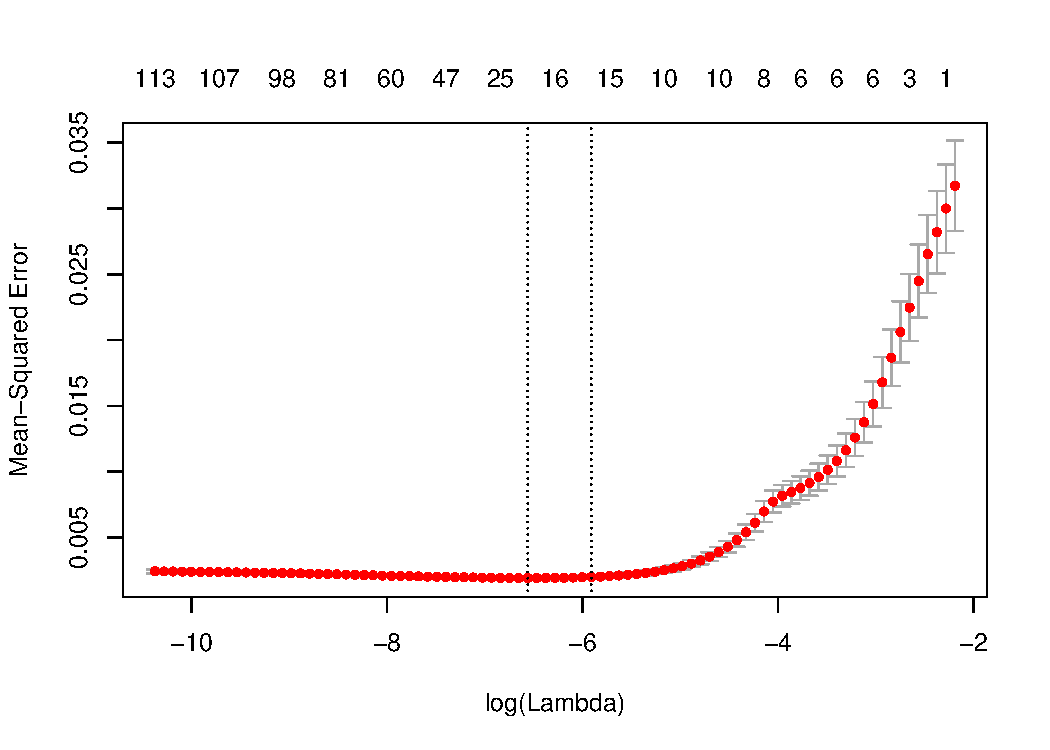
\includegraphics[width=.225\textwidth]{fig/img/lasso_cv.pdf}
%
%
%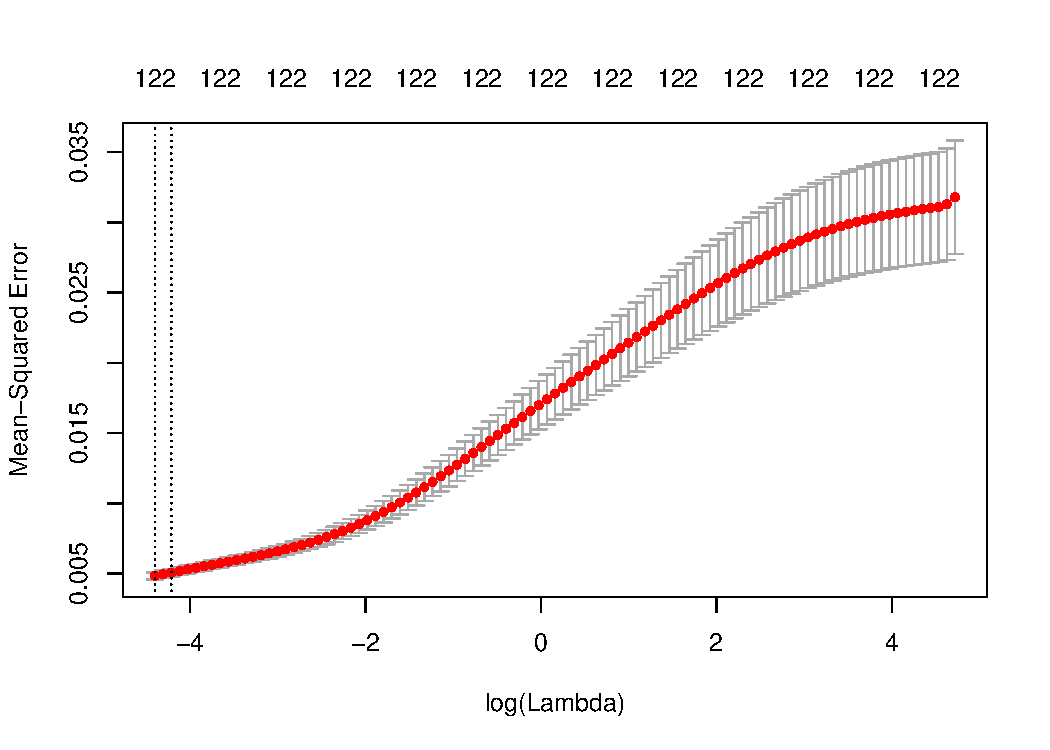
\includegraphics[width=.225\textwidth]{fig/img/ridge_cv.pdf}
%
%\caption{blablabla}
%\label{fig:whatever}
%\end{figure}
%
%
%
%
%Tabellen viser  $\lambda_{min}$ og $\lambda_{\text{1sd}}$ for Ridge regression, lasso og group lasso. 
%
%
%
%
%
%Tabel \ref{tab:cv_lasso} viser værdien af $\lambda_{min}$ og $\lambda_{\text{1sd}}$ samt værdien af $p$, som betegner antallet af parameter og den gennemsnitlige krydsvalideringsfejl. 
%\begin{table}
\center
\begin{tabular}{cccc}
\toprule
\multicolumn{4}{c}{Lasso} \\ \midrule
 & $\lambda$-værdi & fejl &$ p$ \\ \
 $\lambda_{min}$ & 0.0014 & 0.0019 & 20 \\ 
 $\lambda_{1se}$ & 0.0032 & 0.0020 & 15 \\ \bottomrule
\end{tabular}
\caption{Tabellen viser krydsvalideringsfejl samt antal valgte parameter for de to lambda værdier.  } \label{tab:cv_lasso}
\end{table}. 
%Figur \ref{fig:cv_lasso_img} viser forholdet mellem værdierne af logaritmen af $\lambda$, samt krydsvaliderings fejlene. 
%Der ses, at det er først når log lambda er større end -6, der sker nogle signifikante ændringer i krydsvalideringfejlene.
%
%Tabel \ref{tab: lasso_ud} viser hvilken variabler lasso udvælger. Vi kan se, at lasso vælger 9 variabler ud af de 15, som tilhører gruppen arbejdsmarked. 
%
%Figur \ref{fig:cv_lasso_img} viser forholdet mellem værdien af log af lambda, samt krydsvaliderings fejlene. 
%
%\imgfigh{lasso_cv.pdf}{0.7}{Viser krydsvalidering stien, hvor forholdet mellem den gennemsnitlige kvadraters fejl og $\lambda$ værdierne. De lodrette stiplede streger viser logaritmen af $\lambda_min$  og $\lambda_1se$}{cv_lasso_img}
% 
%
%
%\begin{table}
\small
\center
\begin{tabular}{lcc}
\toprule
\multicolumn{2}{c}{Lasso} \\ \midrule
Durable Materials (Output og indkomst) & \\
Ratio of Help Wanted/No. Unemployed (Arbejdsmarked) & \\
Civilian Labor Force (Arbejdsmarked)  & \\
Civilian Employment  (Arbejdsmarked) & \\
Civilian Unemployed - Less Than 5 Weeks (Arbejdsmarked)  & \\
Civilians Unemployed for 5-14 weeks (Arbejdsmarked) & \\
Civilian Unemployed - 15 Weeks \& Over (Arbejdsmarked) & \\
All Employees: Total Nonfarm (Arbejdsmarked) &\\
All Employees: Gods-Producing Industries (Arbejdsmarked) & \\
All Employees: Construction (Arbejdsmarked) & \\
Housing Starts, West (Boliger) & \\
Real Personal Consumption expenditures (Forbrug, ordrer og varebeholdning) &\\
New Orders for Durable Goods (Forbrug, ordrer og varebeholdning)  & \\
5 Years Treasure Rate (Rente og valutakurs) &\\
U.S /U.K Foreign Exchange Rate  (Rente og valutakurs)  & \\ \bottomrule
\end{tabular}
\caption{Overstående er de forklarende variable, som bliver udvalgt af lasso. Det der står i parantes er hvilken gruppe hver variable tilhører} \label{tab: lasso_ud}
\end{table}

%
%
%\subsection{Ridge}
%Vi ved at ridge regression ikke mindsker antallet af forklarende variable, men derimod bare mindsker estimaterne. Derfor lader vi den optimale $\lambda$-værdi være den med mindst krydsvalideringsfejl, siden at $\lambda$ med en standard afvigelse i fejlene vil ikke ændre på kompleksiteten. Dette ses også i tabellen \ref{tab:cv_ridge}. 
%
%\begin{table}
\center
\begin{tabular}{cccc}
\toprule
\multicolumn{4}{c}{Ridge} \\ \midrule
 & $\lambda$-værdi & fejl &$ p$ \\ 
 $\lambda_{min}$ & 0.012 & 0.0048 & 122 \\ 
 $\lambda_{1se}$ & 0.015 & 0.0051 & 122 \\ \bottomrule
\end{tabular}
\caption{Tabellen viser krydsvalideringsfejl samt antal valgte parameter for de to lambda værdier.  } \label{tab:cv_ridge}
\end{table}
%På plottet ses også, at log $\lambda$ ikke skal være meget større end -4 før vi får en høj fejl.
%\imgfigh{ridge_cv.pdf}{0.7}{Viser krydsvalidering stien, hvor forholdet mellem den gennemsnitlige kvadraters fejl og $\lambda$ værdierne. De lodrette stiplede streger viser logaritmen af $\lambda_{min}$  og $\lambda_{1se}$ }{cv_ridge_img}
%
%
%
%\subsection{Elastic Net}
%For elastik net ses i ligning ... , at vi har to ubekendte variable nemlig $\alpha$ og $\lambda$, hvor $\alpha \in [0,1]$. 
%Vi tester derfor en følge med længde 10 af $\alpha$-værdier og ud fra hver værdi af $\alpha$ finder vi $\lambda_{min}$ og $\lambda_{1se}$ og deres gennemsnitlige krydsvaliderings fejl. Disse værdier ses i tabel \ref{tab:cv_el}. 
%
%\begin{table}
\center
\begin{tabular}{lllll}
\toprule
\multicolumn{5}{c}{Elastic net} \\ \midrule
 $\lambda_{\min}$& $\text{kvm}_{\min}$ & $\lambda_{1se}$ & $\text{kvm}_{1se}$ & $\alpha$\  \\
0.0005 & 0.0024 & 0.0011 & 0.0025 & 0.1000 \\
0.0007 & 0.0024 & 0.0017 & 0.0024& 0.1889 \\
0.0010 & 0.0023 & 0.0020 & 0.0024& 0.2778 \\
0.0012 &  0.0022& 0.0022& 0.0023& 0.3667 \\
0.0012& 0.0021& 0.0024 & 0.0022&  0.4556 \\
0.0011 &  0.0021 & 0.0026 & 0.0022 &  0.5444 \\
0.0014 &  0.0021 & 0.0025 &  0.0021& 0.6333 \\
0.0015 & 0.0020 &  0.0026 & 0.0021 & 0.7222 \\
0.0014 &  0.0020 &  0.0023 &  0.0020& 0.8111 \\
0.0013& 0.0019& 0.0027& 0.0020 &  0.9000 \\ \bottomrule
\end{tabular}
\caption{Tabellen viser middelværdien af krydsvalideringsfejlene (kvm) for $\lambda_{\min}$ og $\lambda_{1se}$ for hvert valg af $\alpha$. } \label{tab:cv_el}
\end{table}
%For at få et bedre overblik viser tabel  \ref{tab:cv_el1}  den $\lambda_min$ samt den $\lambda_{1se}$ med mindst gennemsnitlige krydsvalideringsfejl, samt antallet af parameter. 
%Igen ser vi, at krydsvaliderings fejl for $\lambda_{1se}$ ikke er signifikant forskellige fra $\lambda_{\min}$, men der sker en mindskning i kompleksiteten. Derfor vil vores optimale model være modellen med $\lambda_{1se}$. 
%\begin{table}
\center
\begin{tabular}{ccccc}
\toprule
\multicolumn{5}{c}{Elastic Net} \\ \midrule
 & $\lambda$-værdi & kvm & alpha & $p$ \\ 
 $\lambda_{min}$ & 0.0013 & 0.0019 & 0.9 & 23  \\ 
 $\lambda_{1se}$ & 0.015 & 0.0020 & 0.8111 & 19 \\ \bottomrule
\end{tabular}
\caption{Tabellen viser det gennemsnitlige krydsvalideringsfejl (kvm) samt antal valgte parameter for de to lambda værdier.  } \label{tab:cv_el1}
\end{table}
%Tabel \ref{tab: el_ud} viser hvilken variabler elastic net udvælger, som de forklarende variabler. Her kan vi igen se, at de fleste af de udvalgte variabler er i samme gruppe, som vores responsvariable nemlig arbejdsmarked.  
%\begin{table}
\small
\center
\begin{tabular}{lcc}
\toprule
\multicolumn{2}{c}{Elastic Net} \\ \midrule
Duarable Materials (Output og indkomst) & \Duarable Materials (1) \\\
Nondurable Materials (Output og indkomst) &\\
Residential Utilities (Output og indkomst) &\\
Civilian Labor Force (Arbejdsmarked) &\\
Civilian Employment (Arbejdsmarked) &\\
Average Duration of Unemployment (weeks) (Arbejdsmarked) &\\
Civilians Unemployed - Less Than 5 Weeks (Arbejdsmarked) &\\
Civilians Unemployed for 5-14 Weeks (Arbejdsmarked) &\\
Civilians Unemployed- 15 Weeks and Over (Arbejdsmarked)& \\
Intial Claims (Arbejdsmarked) &\\
All Employees: Mining and Logging: Minning (Arbejdsmarked) & \\
All Employees: Construction (Arbejdsmarked) &\\
All Employees:  Wholesale Trade (Arbejdsmarked) &\\
Housing Starts West (Boliger) &\\
Real Personal Consumption Expenditures (Forbrug, ordrer og varebeholdning)& \\
New Orders for Durable Goods (Forbrug, ordrer og varebeholdning)&\\
Nonrevolving consumer credit to Personal Income (Penge og kredit) &\\
5-years Treaury Rate (Rente og Valutakurs) &\\
Japan / U.S Foreign Exchange Rate (Rente og Valutakurs) &\\
U.S / U.K Foreign Exchange Rate (Rente og Valutakurs)& \\
PPI: Intermediate Materials (Priser)& \\
PPI: Metals and metal products:(Priser) &\\
CPI: Mediacal Care (Priser)& \\ \bottomrule
\end{tabular}
\caption{Overstående er de forklarende variable, som bliver udvalgt af elastik net. Det der står i parantes er hvilken gruppe hver variable tilhører} \label{tab: el_ud}
\end{table}

\multicolumn{2}{c}{Elastic Net} \\ \midrule

Nondurable Materials (1) &\\
Residential Utilities (1) &\\
Civilian Labor Force (2) &\\
Civilian Employment (2) &\\
Average Duration of Unemployment (weeks) (2) &\\
Civilians Unemployed - Less Than 5 Weeks (2) &\\
Civilians Unemployed for 5-14 Weeks (2) &\\
Civilians Unemployed- 15 Weeks and Over (2)& \\
Intial Claims (2) &\\
All Employees: Mining and Logging: Minning (2) & \\
All Employees: Construction (2) &\\
All Employees:  Wholesale Trade (2) &\\
Housing Starts West (3) &\\
Real Personal Consumption Expenditures (4) & \\
New Orders for Durable Goods (4)&\\
Nonrevolving consumer credit to Personal Income (5) &\\
5-years Treaury Rate (6) &\\
Japan / U.S Foreign Exchange Rate (6) &\\
U.S / U.K Foreign Exchange Rate (6& \\
PPI: Intermediate Materials (7)& \\
PPI: Metals and metal products:(7) &\\
CPI: Mediacal Care (7)& \\ \bottomrule

%
%
%\subsection{Group Lasso}
%I denne metode anvender vi de inddelte grupper, som tidligere nævnt. 
%Vi får at alle estimaterne bliver valgt, som selvfølgelig indikerer på at metoden ikke passer til vores data. 
%
%\imgfigh{group_cv.pdf}{0.7}{Viser krydsvalidering stien, hvor forholdet mellem den gennemsnitlige kvadraters fejl og $\lambda$ værdierne. De lodrette stiplede streger viser logaritmen af $\lambda_{min}$  og $\lambda_{1se}$ }{group_cv}
%
%
%
%
%
